\documentclass{standalone}
\usepackage{tikz}
\usetikzlibrary{patterns}
\usetikzlibrary{positioning}
\usetikzlibrary{patterns, positioning}
\usetikzlibrary{shapes.misc}
\usepackage[outline]{contour}
\contourlength{1.5pt} 


\begin{document}
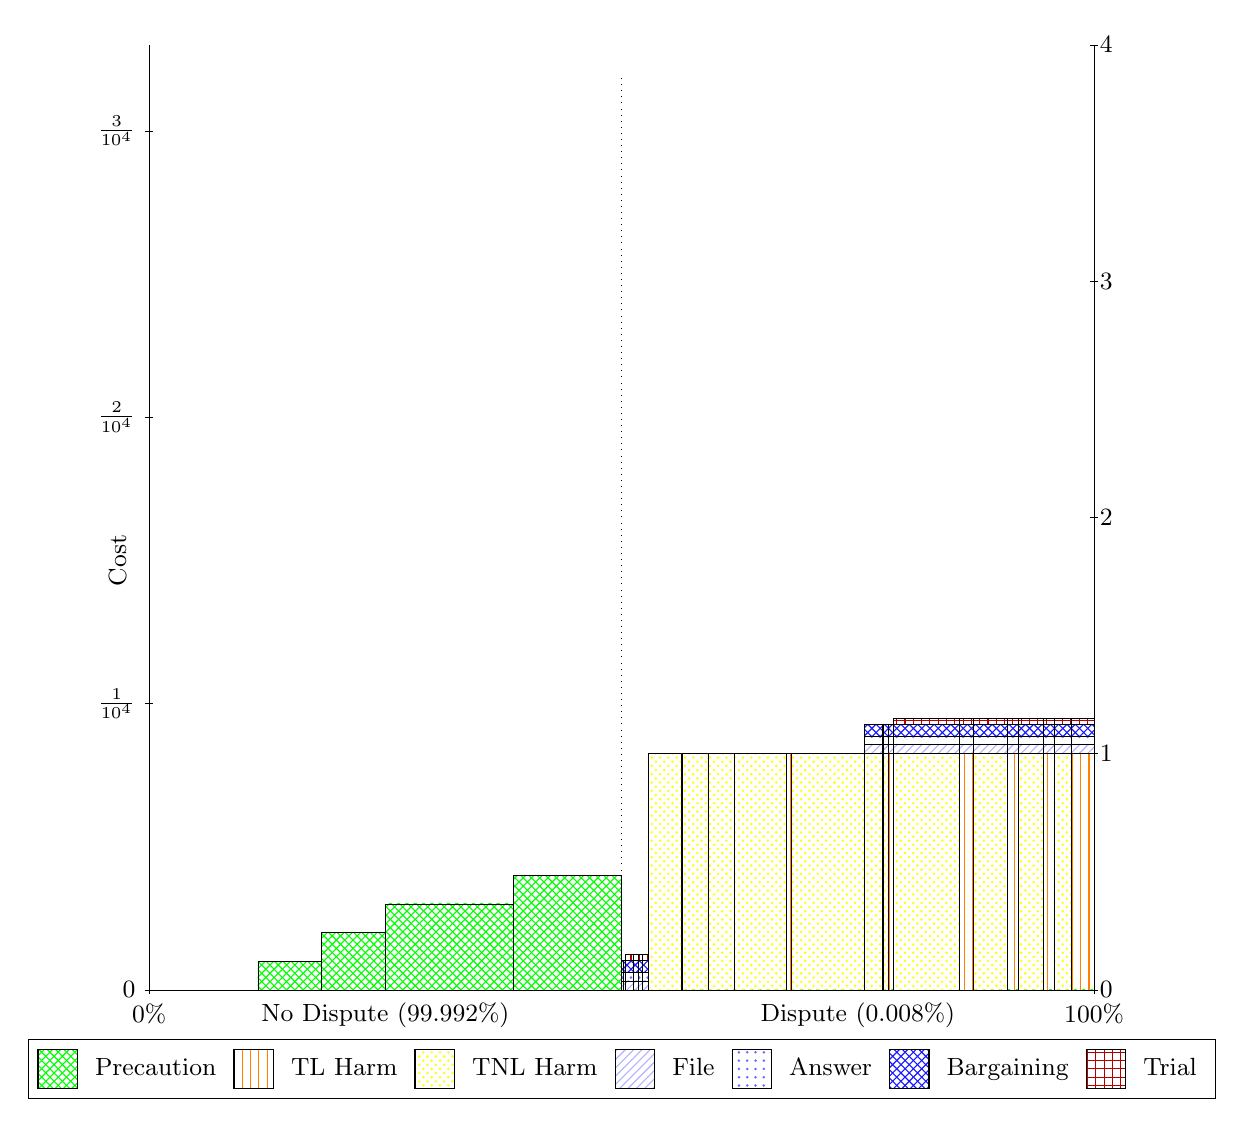
\begin{tikzpicture}
\draw[pattern=crosshatch, pattern color=green,draw=black,very thin] (2.8801,2.5) rectangle (3.6907,2.8636);
\draw[pattern=crosshatch, pattern color=green,draw=black,very thin] (3.6907,2.5) rectangle (4.4999,3.2271);
\draw[pattern=crosshatch, pattern color=green,draw=black,very thin] (4.4999,2.5) rectangle (6.1199,3.5907);
\draw[pattern=crosshatch, pattern color=green,draw=black,very thin] (6.1199,2.5) rectangle (7.5,3.9542);
\draw[pattern=north east lines, pattern color=blue!30,draw=black,very thin] (7.5,2.5) rectangle (7.5234,2.6125);
\draw[pattern=dots,  pattern color=blue!60,draw=black,very thin] (7.5,2.6125) rectangle (7.5234,2.725);
\draw[pattern=crosshatch,      pattern color=blue!90,draw=black,very thin] (7.5,2.725) rectangle (7.5234,2.875);
\draw[pattern=crosshatch, pattern color=green,draw=black,very thin] (7.5234,2.5) rectangle (7.5435,2.5001);
\draw[pattern=north east lines, pattern color=blue!30,draw=black,very thin] (7.5234,2.5001) rectangle (7.5435,2.6126);
\draw[pattern=dots,  pattern color=blue!60,draw=black,very thin] (7.5234,2.6126) rectangle (7.5435,2.7251);
\draw[pattern=crosshatch,      pattern color=blue!90,draw=black,very thin] (7.5234,2.7251) rectangle (7.5435,2.8751);
\draw[pattern=north east lines, pattern color=blue!30,draw=black,very thin] (7.5435,2.5) rectangle (7.645,2.6125);
\draw[pattern=dots,  pattern color=blue!60,draw=black,very thin] (7.5435,2.6125) rectangle (7.645,2.725);
\draw[pattern=crosshatch,      pattern color=blue!90,draw=black,very thin] (7.5435,2.725) rectangle (7.645,2.875);
\draw[pattern=grid,            pattern color=red!70!black,draw=black,very thin] (7.5435,2.875) rectangle (7.645,2.95);
\draw[pattern=crosshatch, pattern color=green,draw=black,very thin] (7.645,2.5) rectangle (7.7072,2.5);
\draw[pattern=north east lines, pattern color=blue!30,draw=black,very thin] (7.645,2.5) rectangle (7.7072,2.6125);
\draw[pattern=dots,  pattern color=blue!60,draw=black,very thin] (7.645,2.6125) rectangle (7.7072,2.725);
\draw[pattern=crosshatch,      pattern color=blue!90,draw=black,very thin] (7.645,2.725) rectangle (7.7072,2.875);
\draw[pattern=grid,            pattern color=red!70!black,draw=black,very thin] (7.645,2.875) rectangle (7.7072,2.95);
\draw[pattern=crosshatch, pattern color=green,draw=black,very thin] (7.7072,2.5) rectangle (7.7652,2.5001);
\draw[pattern=north east lines, pattern color=blue!30,draw=black,very thin] (7.7072,2.5001) rectangle (7.7652,2.6126);
\draw[pattern=dots,  pattern color=blue!60,draw=black,very thin] (7.7072,2.6126) rectangle (7.7652,2.7251);
\draw[pattern=crosshatch,      pattern color=blue!90,draw=black,very thin] (7.7072,2.7251) rectangle (7.7652,2.8751);
\draw[pattern=grid,            pattern color=red!70!black,draw=black,very thin] (7.7072,2.8751) rectangle (7.7652,2.9501);
\draw[pattern=crosshatch, pattern color=green,draw=black,very thin] (7.7652,2.5) rectangle (7.8413,2.5001);
\draw[pattern=north east lines, pattern color=blue!30,draw=black,very thin] (7.7652,2.5001) rectangle (7.8413,2.6126);
\draw[pattern=dots,  pattern color=blue!60,draw=black,very thin] (7.7652,2.6126) rectangle (7.8413,2.7251);
\draw[pattern=crosshatch,      pattern color=blue!90,draw=black,very thin] (7.7652,2.7251) rectangle (7.8413,2.8751);
\draw[pattern=grid,            pattern color=red!70!black,draw=black,very thin] (7.7652,2.8751) rectangle (7.8413,2.9501);
\draw[pattern=crosshatch dots, pattern color=yellow,draw=black,very thin] (7.8413,2.5) rectangle (8.2601,5.5);
\draw[pattern=vertical lines, pattern color=orange,draw=black,very thin] (8.2601,2.5) rectangle (8.2656,5.5);
\draw[pattern=crosshatch, pattern color=green,draw=black,very thin] (8.2656,2.5) rectangle (8.5938,2.5);
\draw[pattern=crosshatch dots, pattern color=yellow,draw=black,very thin] (8.2656,2.5) rectangle (8.5938,5.5);
\draw[pattern=crosshatch, pattern color=green,draw=black,very thin] (8.5938,2.5) rectangle (8.5985,2.5);
\draw[pattern=vertical lines, pattern color=orange,draw=black,very thin] (8.5938,2.5) rectangle (8.5985,5.5);
\draw[pattern=crosshatch, pattern color=green,draw=black,very thin] (8.5985,2.5) rectangle (8.9301,2.5001);
\draw[pattern=crosshatch dots, pattern color=yellow,draw=black,very thin] (8.5985,2.5001) rectangle (8.9301,5.5001);
\draw[pattern=crosshatch, pattern color=green,draw=black,very thin] (8.9301,2.5) rectangle (8.9354,2.5001);
\draw[pattern=vertical lines, pattern color=orange,draw=black,very thin] (8.9301,2.5001) rectangle (8.9354,5.5001);
\draw[pattern=crosshatch, pattern color=green,draw=black,very thin] (8.9354,2.5) rectangle (9.5858,2.5001);
\draw[pattern=crosshatch dots, pattern color=yellow,draw=black,very thin] (8.9354,2.5001) rectangle (9.5858,5.5001);
\draw[pattern=crosshatch, pattern color=green,draw=black,very thin] (9.5858,2.5) rectangle (9.6545,2.5001);
\draw[pattern=vertical lines, pattern color=orange,draw=black,very thin] (9.5858,2.5001) rectangle (9.6545,5.5001);
\draw[pattern=crosshatch, pattern color=green,draw=black,very thin] (9.6545,2.5) rectangle (10.586,2.5001);
\draw[pattern=crosshatch dots, pattern color=yellow,draw=black,very thin] (9.6545,2.5001) rectangle (10.586,5.5001);
\draw[pattern=crosshatch dots, pattern color=yellow,draw=black,very thin] (10.586,2.5) rectangle (10.808,5.5);
\draw[pattern=north east lines, pattern color=blue!30,draw=black,very thin] (10.586,5.5) rectangle (10.808,5.6125);
\draw[pattern=dots,  pattern color=blue!60,draw=black,very thin] (10.586,5.6125) rectangle (10.808,5.725);
\draw[pattern=crosshatch,      pattern color=blue!90,draw=black,very thin] (10.586,5.725) rectangle (10.808,5.875);
\draw[pattern=vertical lines, pattern color=orange,draw=black,very thin] (10.808,2.5) rectangle (10.82,5.5);
\draw[pattern=north east lines, pattern color=blue!30,draw=black,very thin] (10.808,5.5) rectangle (10.82,5.6125);
\draw[pattern=dots,  pattern color=blue!60,draw=black,very thin] (10.808,5.6125) rectangle (10.82,5.725);
\draw[pattern=crosshatch,      pattern color=blue!90,draw=black,very thin] (10.808,5.725) rectangle (10.82,5.875);
\draw[pattern=crosshatch, pattern color=green,draw=black,very thin] (10.82,2.5) rectangle (10.891,2.5001);
\draw[pattern=crosshatch dots, pattern color=yellow,draw=black,very thin] (10.82,2.5001) rectangle (10.891,5.5001);
\draw[pattern=north east lines, pattern color=blue!30,draw=black,very thin] (10.82,5.5001) rectangle (10.891,5.6126);
\draw[pattern=dots,  pattern color=blue!60,draw=black,very thin] (10.82,5.6126) rectangle (10.891,5.7251);
\draw[pattern=crosshatch,      pattern color=blue!90,draw=black,very thin] (10.82,5.7251) rectangle (10.891,5.8751);
\draw[pattern=crosshatch, pattern color=green,draw=black,very thin] (10.891,2.5) rectangle (10.954,2.5001);
\draw[pattern=vertical lines, pattern color=orange,draw=black,very thin] (10.891,2.5001) rectangle (10.954,5.5001);
\draw[pattern=north east lines, pattern color=blue!30,draw=black,very thin] (10.891,5.5001) rectangle (10.954,5.6126);
\draw[pattern=dots,  pattern color=blue!60,draw=black,very thin] (10.891,5.6126) rectangle (10.954,5.7251);
\draw[pattern=crosshatch,      pattern color=blue!90,draw=black,very thin] (10.891,5.7251) rectangle (10.954,5.8751);
\draw[pattern=crosshatch dots, pattern color=yellow,draw=black,very thin] (10.954,2.5) rectangle (11.786,5.5);
\draw[pattern=north east lines, pattern color=blue!30,draw=black,very thin] (10.954,5.5) rectangle (11.786,5.6125);
\draw[pattern=dots,  pattern color=blue!60,draw=black,very thin] (10.954,5.6125) rectangle (11.786,5.725);
\draw[pattern=crosshatch,      pattern color=blue!90,draw=black,very thin] (10.954,5.725) rectangle (11.786,5.875);
\draw[pattern=grid,            pattern color=red!70!black,draw=black,very thin] (10.954,5.875) rectangle (11.786,5.95);
\draw[pattern=vertical lines, pattern color=orange,draw=black,very thin] (11.786,2.5) rectangle (11.969,5.5);
\draw[pattern=north east lines, pattern color=blue!30,draw=black,very thin] (11.786,5.5) rectangle (11.969,5.6125);
\draw[pattern=dots,  pattern color=blue!60,draw=black,very thin] (11.786,5.6125) rectangle (11.969,5.725);
\draw[pattern=crosshatch,      pattern color=blue!90,draw=black,very thin] (11.786,5.725) rectangle (11.969,5.875);
\draw[pattern=grid,            pattern color=red!70!black,draw=black,very thin] (11.786,5.875) rectangle (11.969,5.95);
\draw[pattern=crosshatch, pattern color=green,draw=black,very thin] (11.969,2.5) rectangle (12.394,2.5);
\draw[pattern=crosshatch dots, pattern color=yellow,draw=black,very thin] (11.969,2.5) rectangle (12.394,5.5);
\draw[pattern=north east lines, pattern color=blue!30,draw=black,very thin] (11.969,5.5) rectangle (12.394,5.6125);
\draw[pattern=dots,  pattern color=blue!60,draw=black,very thin] (11.969,5.6125) rectangle (12.394,5.725);
\draw[pattern=crosshatch,      pattern color=blue!90,draw=black,very thin] (11.969,5.725) rectangle (12.394,5.875);
\draw[pattern=grid,            pattern color=red!70!black,draw=black,very thin] (11.969,5.875) rectangle (12.394,5.95);
\draw[pattern=crosshatch, pattern color=green,draw=black,very thin] (12.394,2.5) rectangle (12.533,2.5);
\draw[pattern=vertical lines, pattern color=orange,draw=black,very thin] (12.394,2.5) rectangle (12.533,5.5);
\draw[pattern=north east lines, pattern color=blue!30,draw=black,very thin] (12.394,5.5) rectangle (12.533,5.6125);
\draw[pattern=dots,  pattern color=blue!60,draw=black,very thin] (12.394,5.6125) rectangle (12.533,5.725);
\draw[pattern=crosshatch,      pattern color=blue!90,draw=black,very thin] (12.394,5.725) rectangle (12.533,5.875);
\draw[pattern=grid,            pattern color=red!70!black,draw=black,very thin] (12.394,5.875) rectangle (12.533,5.95);
\draw[pattern=crosshatch, pattern color=green,draw=black,very thin] (12.533,2.5) rectangle (12.86,2.5001);
\draw[pattern=crosshatch dots, pattern color=yellow,draw=black,very thin] (12.533,2.5001) rectangle (12.86,5.5001);
\draw[pattern=north east lines, pattern color=blue!30,draw=black,very thin] (12.533,5.5001) rectangle (12.86,5.6126);
\draw[pattern=dots,  pattern color=blue!60,draw=black,very thin] (12.533,5.6126) rectangle (12.86,5.7251);
\draw[pattern=crosshatch,      pattern color=blue!90,draw=black,very thin] (12.533,5.7251) rectangle (12.86,5.8751);
\draw[pattern=grid,            pattern color=red!70!black,draw=black,very thin] (12.533,5.8751) rectangle (12.86,5.9501);
\draw[pattern=crosshatch, pattern color=green,draw=black,very thin] (12.86,2.5) rectangle (12.996,2.5001);
\draw[pattern=vertical lines, pattern color=orange,draw=black,very thin] (12.86,2.5001) rectangle (12.996,5.5001);
\draw[pattern=north east lines, pattern color=blue!30,draw=black,very thin] (12.86,5.5001) rectangle (12.996,5.6126);
\draw[pattern=dots,  pattern color=blue!60,draw=black,very thin] (12.86,5.6126) rectangle (12.996,5.7251);
\draw[pattern=crosshatch,      pattern color=blue!90,draw=black,very thin] (12.86,5.7251) rectangle (12.996,5.8751);
\draw[pattern=grid,            pattern color=red!70!black,draw=black,very thin] (12.86,5.8751) rectangle (12.996,5.9501);
\draw[pattern=crosshatch, pattern color=green,draw=black,very thin] (12.996,2.5) rectangle (13.215,2.5001);
\draw[pattern=crosshatch dots, pattern color=yellow,draw=black,very thin] (12.996,2.5001) rectangle (13.215,5.5001);
\draw[pattern=north east lines, pattern color=blue!30,draw=black,very thin] (12.996,5.5001) rectangle (13.215,5.6126);
\draw[pattern=dots,  pattern color=blue!60,draw=black,very thin] (12.996,5.6126) rectangle (13.215,5.7251);
\draw[pattern=crosshatch,      pattern color=blue!90,draw=black,very thin] (12.996,5.7251) rectangle (13.215,5.8751);
\draw[pattern=grid,            pattern color=red!70!black,draw=black,very thin] (12.996,5.8751) rectangle (13.215,5.9501);
\draw[pattern=crosshatch, pattern color=green,draw=black,very thin] (13.215,2.5) rectangle (13.5,2.5001);
\draw[pattern=vertical lines, pattern color=orange,draw=black,very thin] (13.215,2.5001) rectangle (13.5,5.5001);
\draw[pattern=north east lines, pattern color=blue!30,draw=black,very thin] (13.215,5.5001) rectangle (13.5,5.6126);
\draw[pattern=dots,  pattern color=blue!60,draw=black,very thin] (13.215,5.6126) rectangle (13.5,5.7251);
\draw[pattern=crosshatch,      pattern color=blue!90,draw=black,very thin] (13.215,5.7251) rectangle (13.5,5.8751);
\draw[pattern=grid,            pattern color=red!70!black,draw=black,very thin] (13.215,5.8751) rectangle (13.5,5.9501);
\draw[black,very thin] (1.5,2.5) -- (1.5,14.5);
\node[font=\small,rotate=90,text=black, anchor=center] at (1.1, 7.9534) {Cost};
\draw[black,very thin] (1.45,2.5) -- (1.55,2.5);
\node[font=\small,text=black, anchor=east] at (1.45, 2.5) {0};
\draw[black,very thin] (1.45,6.1356) -- (1.55,6.1356);
\node[font=\small,text=black, anchor=east] at (1.45, 6.1356) {$\frac{1}{10^{4}}$};
\draw[black,very thin] (1.45,9.7712) -- (1.55,9.7712);
\node[font=\small,text=black, anchor=east] at (1.45, 9.7712) {$\frac{2}{10^{4}}$};
\draw[black,very thin] (1.45,13.407) -- (1.55,13.407);
\node[font=\small,text=black, anchor=east] at (1.45, 13.407) {$\frac{3}{10^{4}}$};

\draw[black,dotted,very thin] (7.5,2.86) -- (7.5,14.14);
\draw[black,very thin] (13.5,2.5) -- (13.5,14.5);
\draw[black,very thin] (13.45,2.5) -- (13.55,2.5);
\node[font=\small,text=black, anchor=west] at (13.45, 2.5) {0};
\draw[black,very thin] (13.45,5.5) -- (13.55,5.5);
\node[font=\small,text=black, anchor=west] at (13.45, 5.5) {1};
\draw[black,very thin] (13.45,8.5) -- (13.55,8.5);
\node[font=\small,text=black, anchor=west] at (13.45, 8.5) {2};
\draw[black,very thin] (13.45,11.5) -- (13.55,11.5);
\node[font=\small,text=black, anchor=west] at (13.45, 11.5) {3};
\draw[black,very thin] (13.45,14.5) -- (13.55,14.5);
\node[font=\small,text=black, anchor=west] at (13.45, 14.5) {4};

\draw[black,very thin] (1.5,2.5) -- (13.5,2.5);
\draw[black,very thin] (1.5,2.45) -- (1.5,2.55);
\node[font=\small,text=black, anchor=north] at (1.5, 2.45) {0\%};
\draw[black,very thin] (13.5,2.45) -- (13.5,2.55);
\node[font=\small,text=black, anchor=north] at (13.5, 2.45) {100\%};

\node[font=\small,text=black,anchor=south] at (4.5, 1.9) {No\ Dispute\ (99.992\%)};
\node[font=\small,text=black,anchor=south] at (10.5, 1.9) {Dispute\ (0.008\%)};
\draw (7.5,2.5) node (B) {};
\begin{scope}[align=center]
\matrix[scale=0.5,draw=black,below=0.5cm of B,nodes={draw},column sep=0.1cm]{
\node[rectangle,draw,minimum width=0.5cm,minimum height=0.5cm,pattern=crosshatch, pattern color=green]{}; & \node[draw=none,font=\small,text=black]{Precaution}; &
\node[rectangle,draw,minimum width=0.5cm,minimum height=0.5cm,pattern=vertical lines, pattern color=orange]{}; & \node[draw=none,font=\small,text=black]{TL Harm}; &
\node[rectangle,draw,minimum width=0.5cm,minimum height=0.5cm,pattern=crosshatch dots, pattern color=yellow]{}; & \node[draw=none,font=\small,text=black]{TNL Harm}; &
\node[rectangle,draw,minimum width=0.5cm,minimum height=0.5cm,pattern=north east lines, pattern color=blue!30]{}; & \node[draw=none,font=\small,text=black]{File}; &
\node[rectangle,draw,minimum width=0.5cm,minimum height=0.5cm,pattern=dots,  pattern color=blue!60]{}; & \node[draw=none,font=\small,text=black]{Answer}; &
\node[rectangle,draw,minimum width=0.5cm,minimum height=0.5cm,pattern=crosshatch,      pattern color=blue!90]{}; & \node[draw=none,font=\small,text=black]{Bargaining}; &
\node[rectangle,draw,minimum width=0.5cm,minimum height=0.5cm,pattern=grid,            pattern color=red!70!black]{}; & \node[draw=none,font=\small,text=black]{Trial}; \\\\
};\end{scope}

\end{tikzpicture}
\end{document}